\section{Works Done}
\label{sec:worksDone}
\subsection{Food Tank Construction}
Food tank is the unit to store food and feed cat whenever required. The tank design was done in the first week and implemented this week. Figure \ref{fig:mamaKabi} shows the look of tank from different viewpoints. A motor will be mounted to the bottom part of the tank so that trigger mechanism can easily control the flow of food. Since there is no cat food present at the moment, the test stage will be handled next week.

\begin{figure}[h]
    \centering
    \begin{subfigure}[b]{0.49\textwidth}
        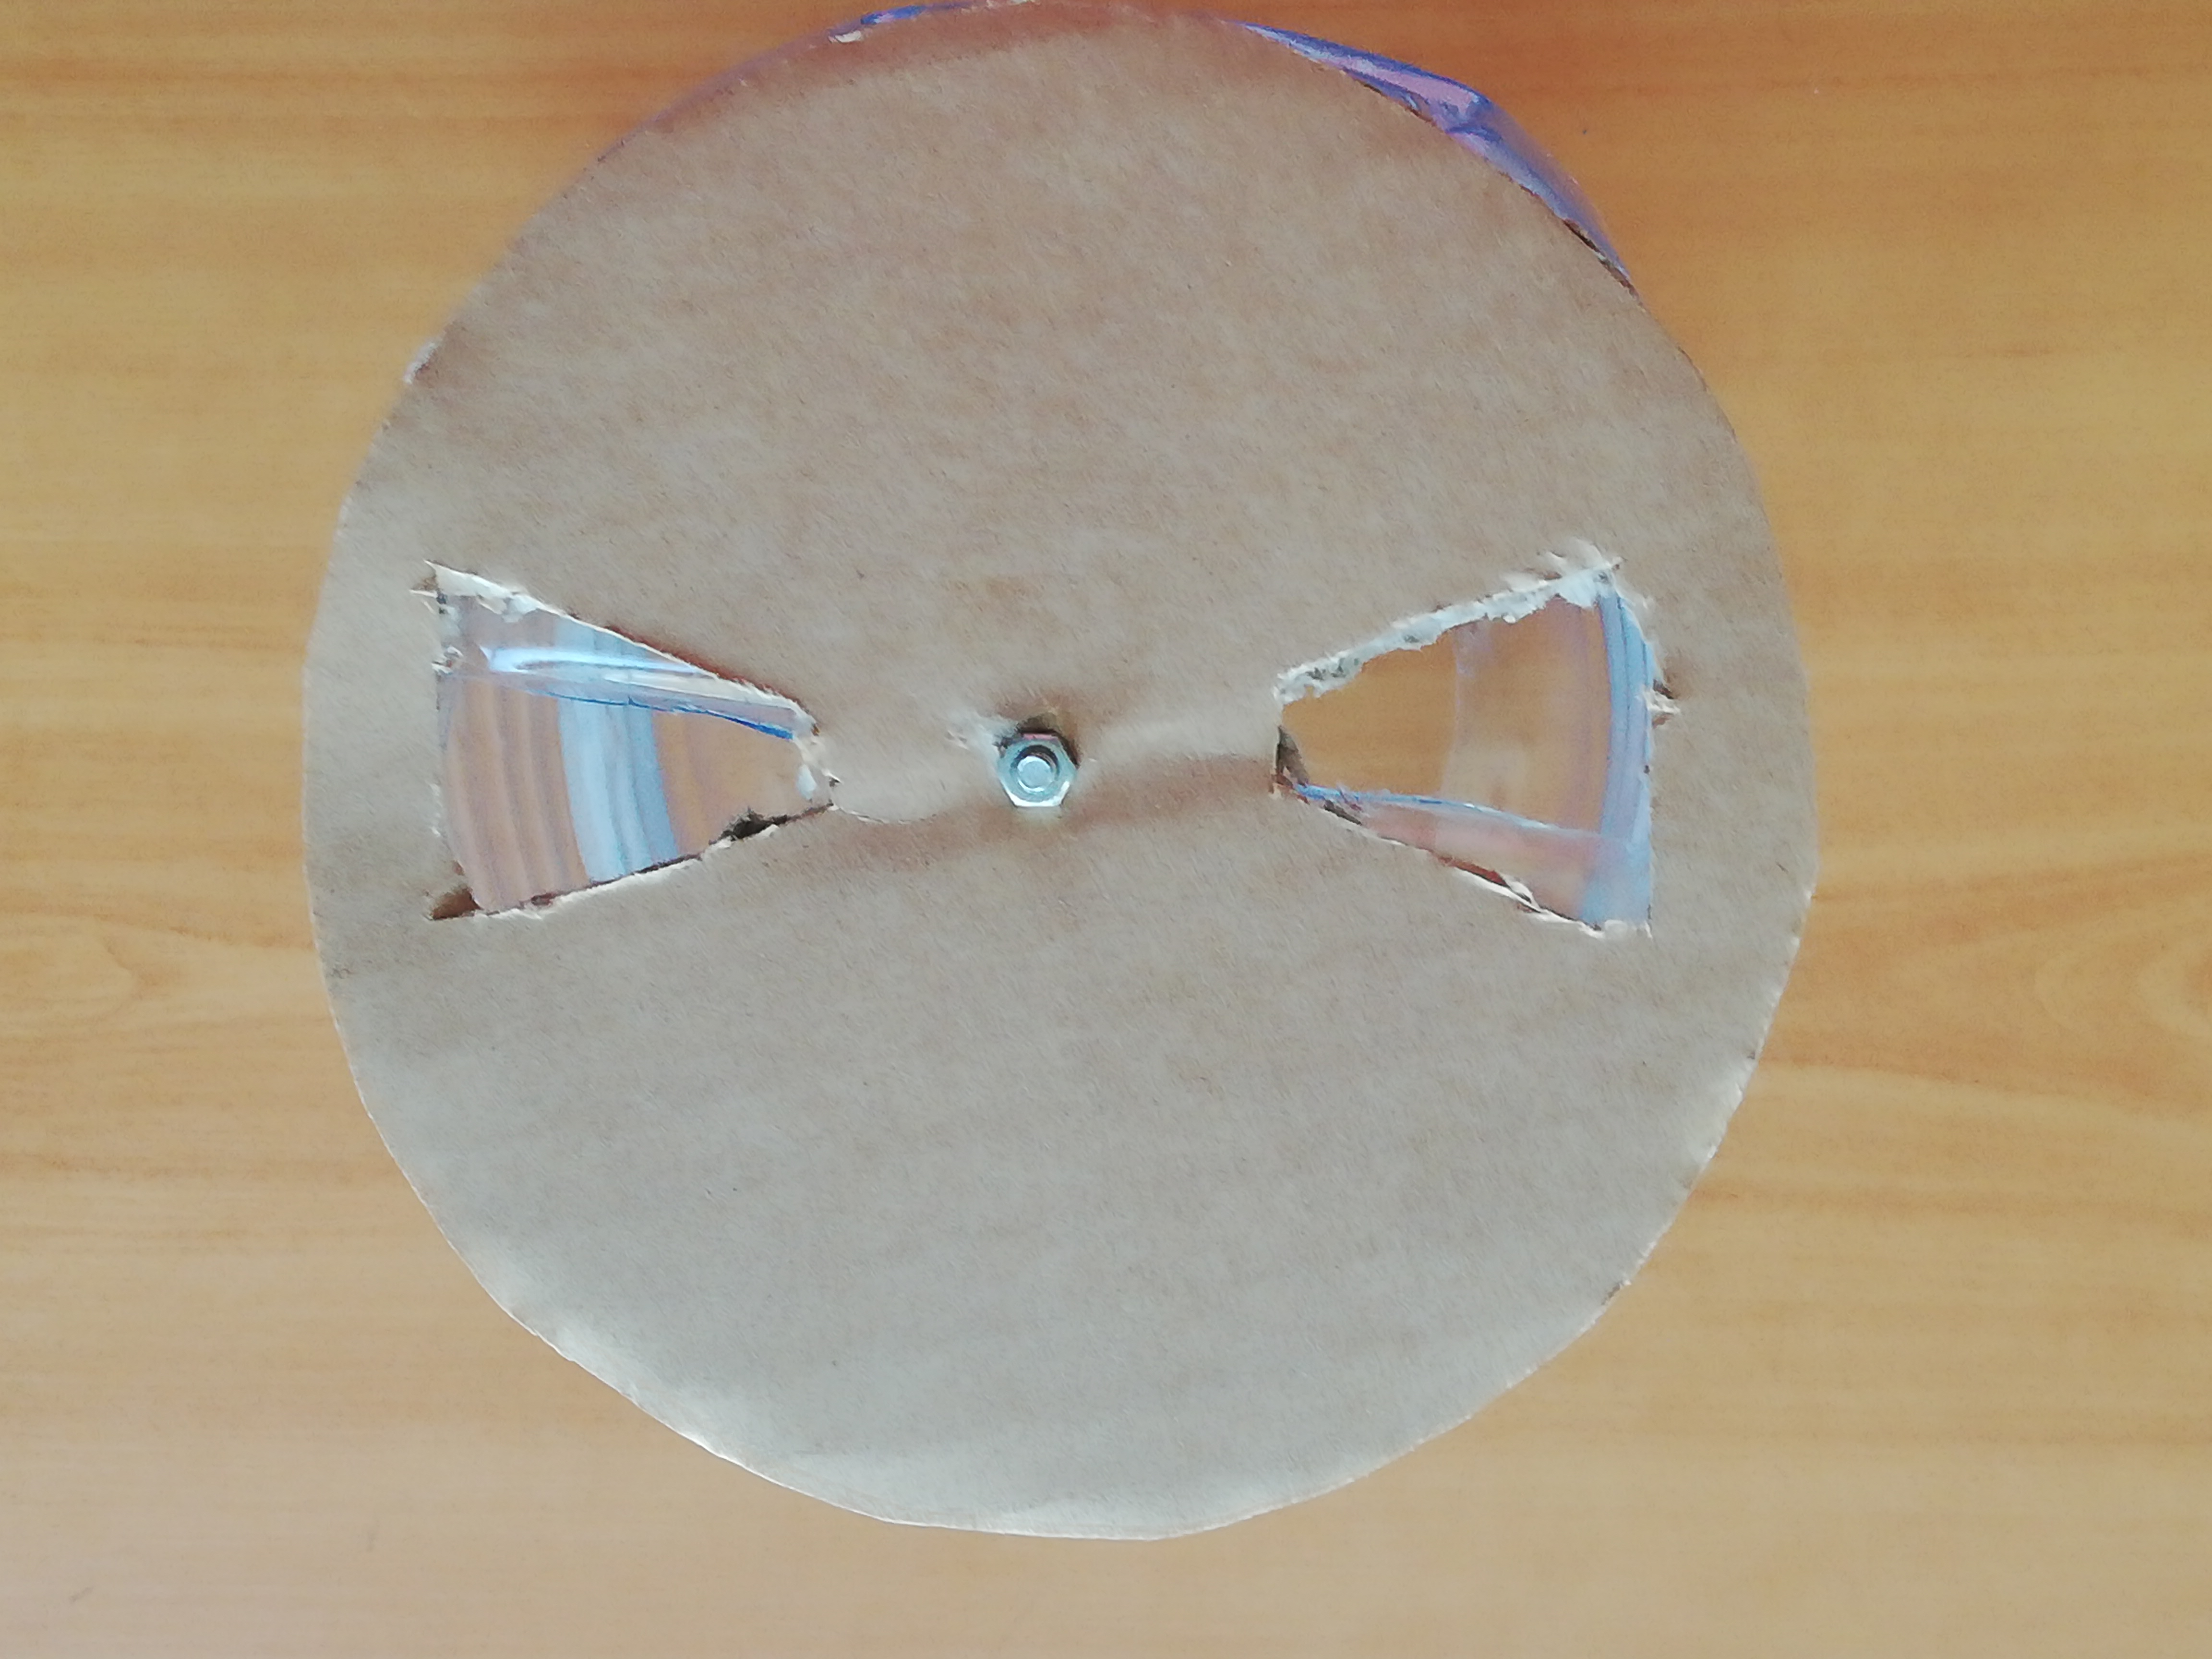
\includegraphics[width=\textwidth]{img/tank1.jpg}
        \caption{Top View}
        \label{fig:mamaKabi1}
    \end{subfigure}
    \begin{subfigure}[b]{0.49\textwidth}
        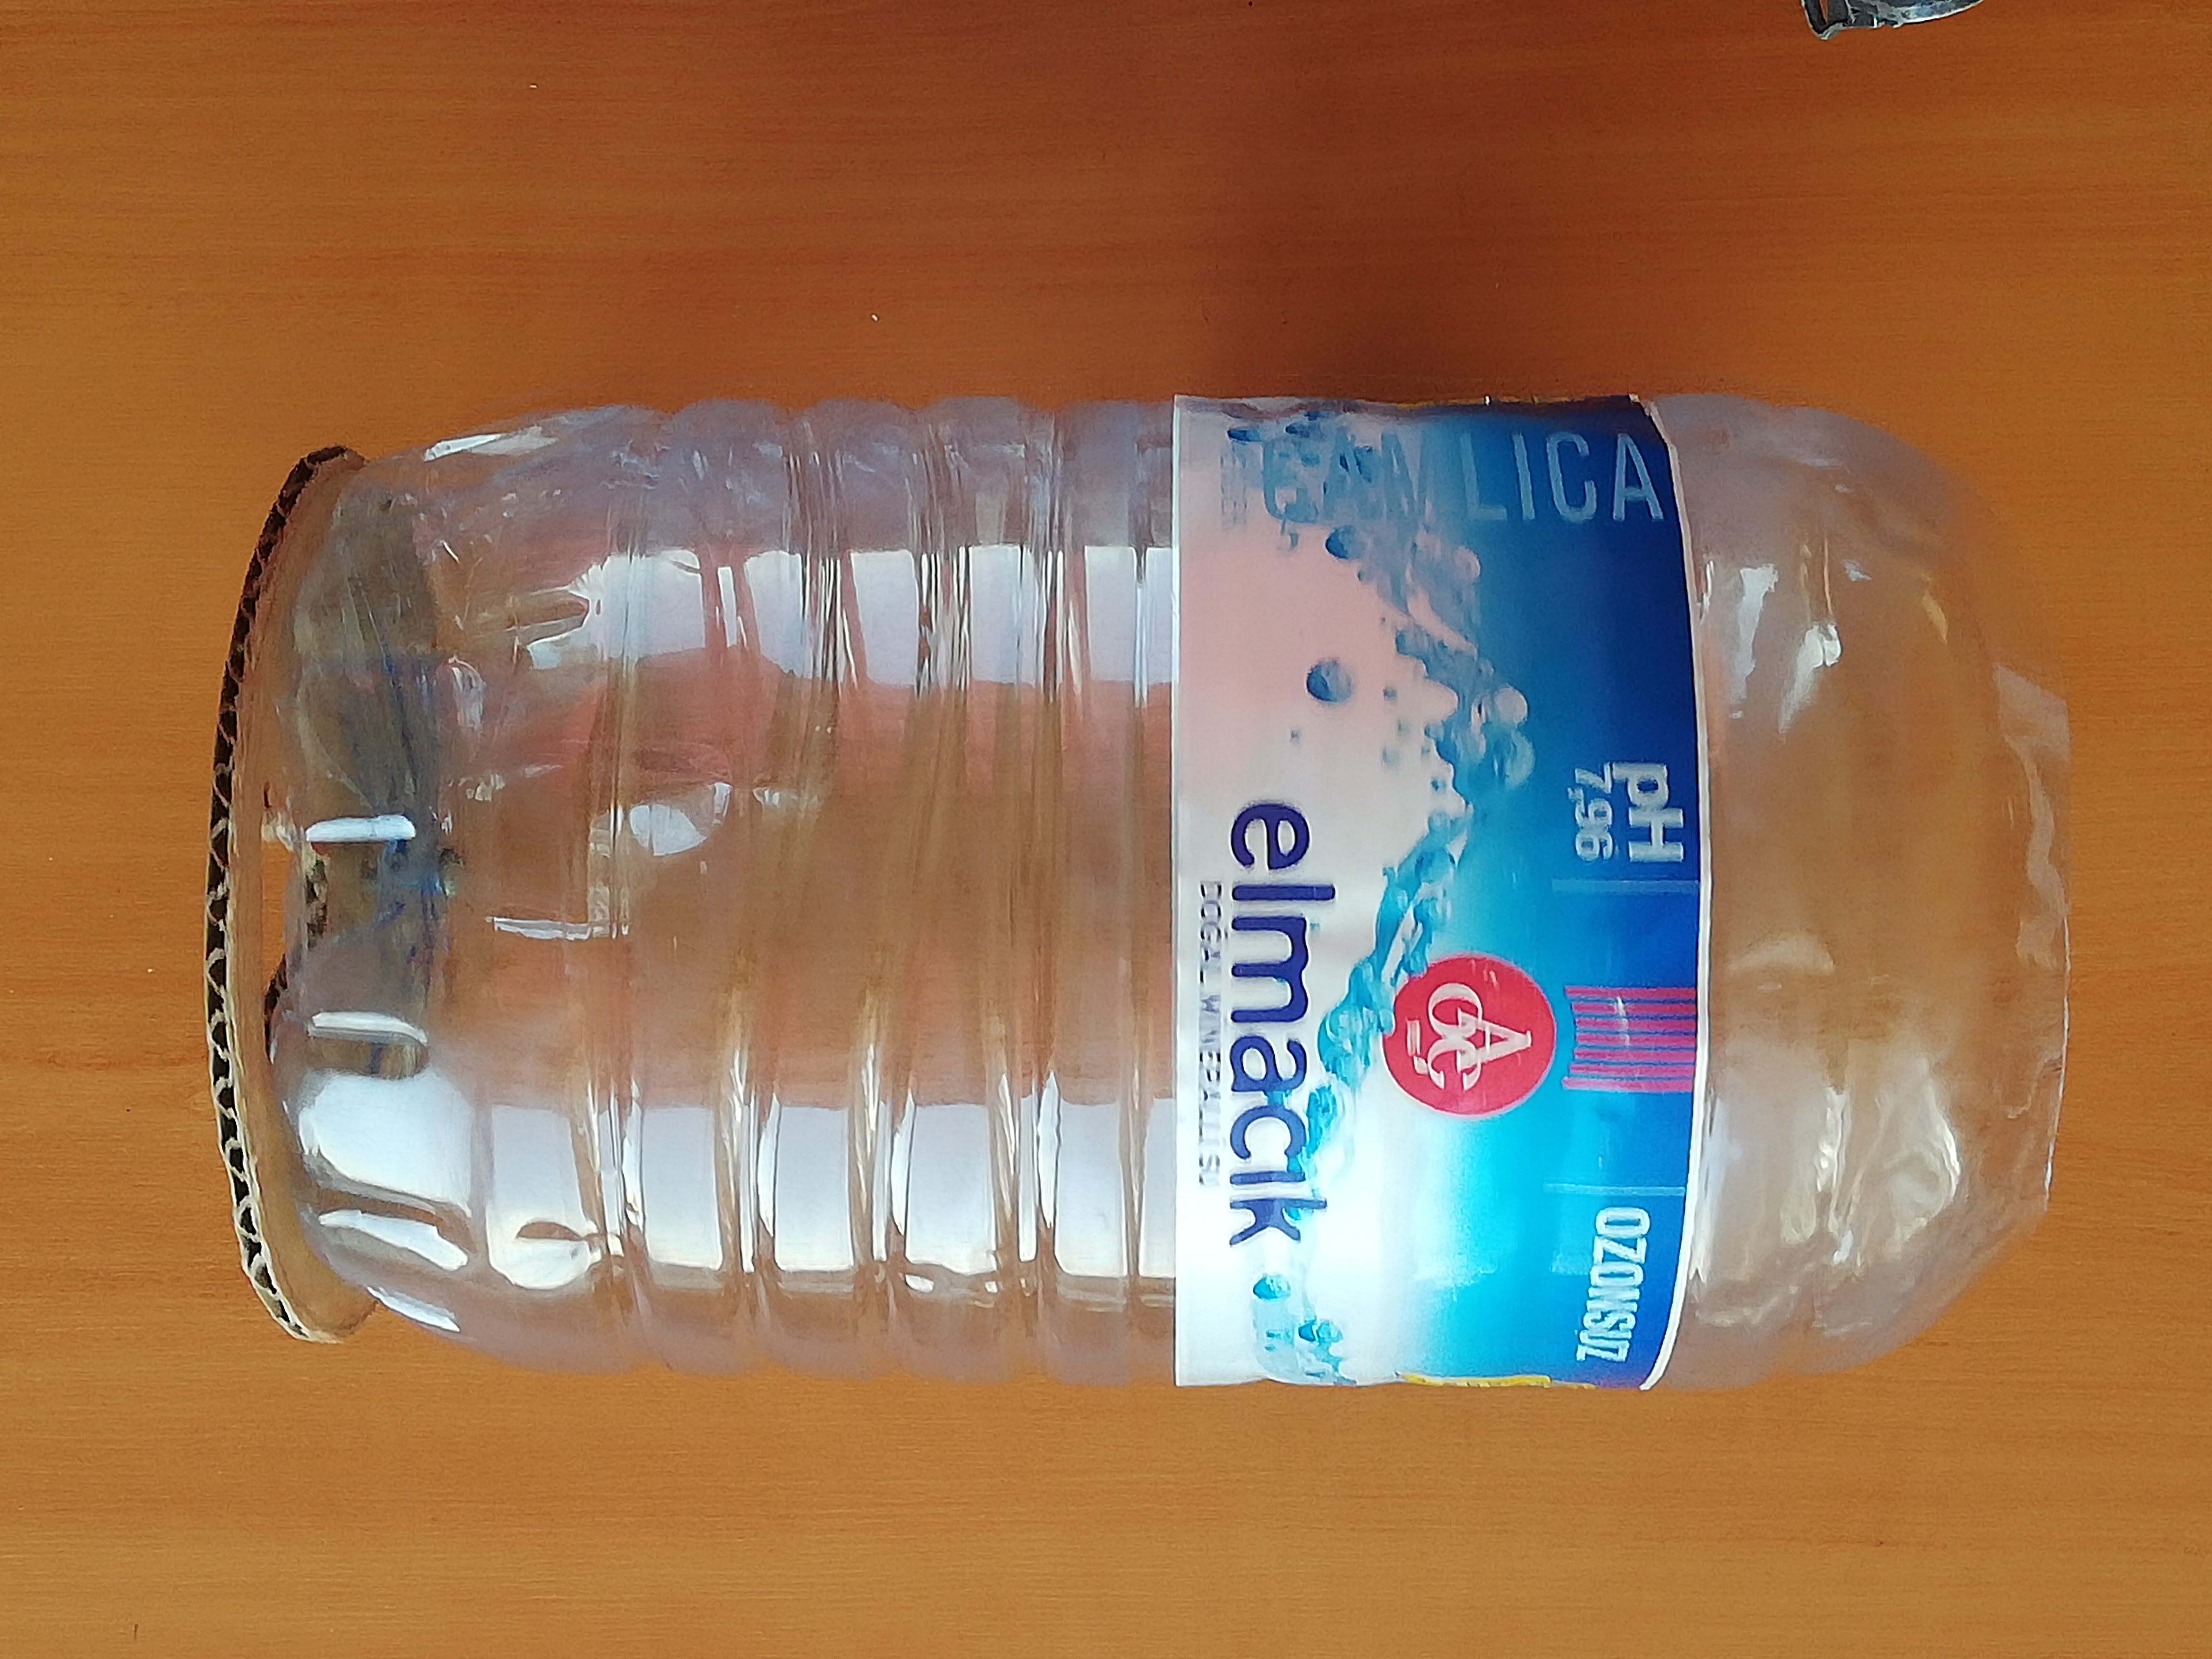
\includegraphics[width=\textwidth]{img/tank2.jpg}
        \caption{Lateral View}
        \label{fig:mamaKabi2}
    \end{subfigure}
    \begin{subfigure}[b]{0.49\textwidth}
        \includegraphics[width=\textwidth]{img/tank3.jpg}
        \caption{Bottom View}
        \label{fig:mamaKabi3}
    \end{subfigure}
     \begin{subfigure}[b]{0.49\textwidth}
        \includegraphics[width=\textwidth]{img/tank4.jpg}
        \caption{Angled View}
        \label{fig:mamaKabi4} 
    \end{subfigure}
    \caption{Food Tank}
    \label{fig:mamaKabi}
\end{figure}

\subsection{Preparing The Computer Vision Environment}
Each team member installed the required software and environment onto their personal computers. Moreover, registrations to cloud computing platforms were done with student packages from the GitHub Student Pack utility\cite{cite:github_studentPack}. \\

Installation of the following packages done : 
\begin{itemize}
    \item Python
    \item Anaconda
    \item OpenCV
\end{itemize}

\subsection{Testing of the Environments}

\begin{itemize}
    \item Online guides \cite{cite:OCV} were used for installation and testing. To test the OpenCV installation, Windows PowerShell (or the command prompt) was used.
    \item Both OpenCV and Python were tested by a simple Web Camera Test \cite{cite:WCT}. This script activates the camera module of the laptop and converts the colored recording to gray by importing CV video capturing functions and running the code on Python. 
    \item As Python editors, the following environments were explored: PyCharm, Visual Studio Code, Spyder, plain old Notepad and the Python terminal. Some were unnecessarily complex, some were unclear; VS Code was eventually seen fit for the purpose.
    
    \item The above mentioned Camera Test was also tried with Anaconda; however, it didn't work because of OpenCV. (This issue will be resolved later since it is not crucial at this step.)
\end{itemize}

\subsection{Proposal Report}

This week's main topic is writing a proposal report. Therefore, a meeting is conducted. In this meeting, we determined the necessary parameters in order to write the proposal report. Moreover, the topics are distributed among the group members and everyone wrote their part. After everyone had written their part, we checked the proposal report again and determined our faults, then brainstorming is done and we corrected our mistakes. 

Proposal report was important for us in order to see ahead, since we have planned the upcoming tasks. Making a Gantt Chart and Weighted Object Tree is important since they enable us to see our future. In the Gantt Chart, we determined the starting and finishing dates of our project and in Weighted Object Tree, we determined the important design parameters of our system. Determining the design parameters is very important since it will be our guide to building our product.
